% Options for packages loaded elsewhere
\PassOptionsToPackage{unicode}{hyperref}
\PassOptionsToPackage{hyphens}{url}
%
\documentclass[
]{article}
\usepackage{amsmath,amssymb}
\usepackage{lmodern}
\usepackage{ifxetex,ifluatex}
\ifnum 0\ifxetex 1\fi\ifluatex 1\fi=0 % if pdftex
  \usepackage[T1]{fontenc}
  \usepackage[utf8]{inputenc}
  \usepackage{textcomp} % provide euro and other symbols
\else % if luatex or xetex
  \usepackage{unicode-math}
  \defaultfontfeatures{Scale=MatchLowercase}
  \defaultfontfeatures[\rmfamily]{Ligatures=TeX,Scale=1}
\fi
% Use upquote if available, for straight quotes in verbatim environments
\IfFileExists{upquote.sty}{\usepackage{upquote}}{}
\IfFileExists{microtype.sty}{% use microtype if available
  \usepackage[]{microtype}
  \UseMicrotypeSet[protrusion]{basicmath} % disable protrusion for tt fonts
}{}
\makeatletter
\@ifundefined{KOMAClassName}{% if non-KOMA class
  \IfFileExists{parskip.sty}{%
    \usepackage{parskip}
  }{% else
    \setlength{\parindent}{0pt}
    \setlength{\parskip}{6pt plus 2pt minus 1pt}}
}{% if KOMA class
  \KOMAoptions{parskip=half}}
\makeatother
\usepackage{xcolor}
\IfFileExists{xurl.sty}{\usepackage{xurl}}{} % add URL line breaks if available
\IfFileExists{bookmark.sty}{\usepackage{bookmark}}{\usepackage{hyperref}}
\hypersetup{
  pdftitle={R Module 4},
  pdfauthor={GHY 5800},
  hidelinks,
  pdfcreator={LaTeX via pandoc}}
\urlstyle{same} % disable monospaced font for URLs
\usepackage[margin=1in]{geometry}
\usepackage{color}
\usepackage{fancyvrb}
\newcommand{\VerbBar}{|}
\newcommand{\VERB}{\Verb[commandchars=\\\{\}]}
\DefineVerbatimEnvironment{Highlighting}{Verbatim}{commandchars=\\\{\}}
% Add ',fontsize=\small' for more characters per line
\usepackage{framed}
\definecolor{shadecolor}{RGB}{248,248,248}
\newenvironment{Shaded}{\begin{snugshade}}{\end{snugshade}}
\newcommand{\AlertTok}[1]{\textcolor[rgb]{0.94,0.16,0.16}{#1}}
\newcommand{\AnnotationTok}[1]{\textcolor[rgb]{0.56,0.35,0.01}{\textbf{\textit{#1}}}}
\newcommand{\AttributeTok}[1]{\textcolor[rgb]{0.77,0.63,0.00}{#1}}
\newcommand{\BaseNTok}[1]{\textcolor[rgb]{0.00,0.00,0.81}{#1}}
\newcommand{\BuiltInTok}[1]{#1}
\newcommand{\CharTok}[1]{\textcolor[rgb]{0.31,0.60,0.02}{#1}}
\newcommand{\CommentTok}[1]{\textcolor[rgb]{0.56,0.35,0.01}{\textit{#1}}}
\newcommand{\CommentVarTok}[1]{\textcolor[rgb]{0.56,0.35,0.01}{\textbf{\textit{#1}}}}
\newcommand{\ConstantTok}[1]{\textcolor[rgb]{0.00,0.00,0.00}{#1}}
\newcommand{\ControlFlowTok}[1]{\textcolor[rgb]{0.13,0.29,0.53}{\textbf{#1}}}
\newcommand{\DataTypeTok}[1]{\textcolor[rgb]{0.13,0.29,0.53}{#1}}
\newcommand{\DecValTok}[1]{\textcolor[rgb]{0.00,0.00,0.81}{#1}}
\newcommand{\DocumentationTok}[1]{\textcolor[rgb]{0.56,0.35,0.01}{\textbf{\textit{#1}}}}
\newcommand{\ErrorTok}[1]{\textcolor[rgb]{0.64,0.00,0.00}{\textbf{#1}}}
\newcommand{\ExtensionTok}[1]{#1}
\newcommand{\FloatTok}[1]{\textcolor[rgb]{0.00,0.00,0.81}{#1}}
\newcommand{\FunctionTok}[1]{\textcolor[rgb]{0.00,0.00,0.00}{#1}}
\newcommand{\ImportTok}[1]{#1}
\newcommand{\InformationTok}[1]{\textcolor[rgb]{0.56,0.35,0.01}{\textbf{\textit{#1}}}}
\newcommand{\KeywordTok}[1]{\textcolor[rgb]{0.13,0.29,0.53}{\textbf{#1}}}
\newcommand{\NormalTok}[1]{#1}
\newcommand{\OperatorTok}[1]{\textcolor[rgb]{0.81,0.36,0.00}{\textbf{#1}}}
\newcommand{\OtherTok}[1]{\textcolor[rgb]{0.56,0.35,0.01}{#1}}
\newcommand{\PreprocessorTok}[1]{\textcolor[rgb]{0.56,0.35,0.01}{\textit{#1}}}
\newcommand{\RegionMarkerTok}[1]{#1}
\newcommand{\SpecialCharTok}[1]{\textcolor[rgb]{0.00,0.00,0.00}{#1}}
\newcommand{\SpecialStringTok}[1]{\textcolor[rgb]{0.31,0.60,0.02}{#1}}
\newcommand{\StringTok}[1]{\textcolor[rgb]{0.31,0.60,0.02}{#1}}
\newcommand{\VariableTok}[1]{\textcolor[rgb]{0.00,0.00,0.00}{#1}}
\newcommand{\VerbatimStringTok}[1]{\textcolor[rgb]{0.31,0.60,0.02}{#1}}
\newcommand{\WarningTok}[1]{\textcolor[rgb]{0.56,0.35,0.01}{\textbf{\textit{#1}}}}
\usepackage{graphicx}
\makeatletter
\def\maxwidth{\ifdim\Gin@nat@width>\linewidth\linewidth\else\Gin@nat@width\fi}
\def\maxheight{\ifdim\Gin@nat@height>\textheight\textheight\else\Gin@nat@height\fi}
\makeatother
% Scale images if necessary, so that they will not overflow the page
% margins by default, and it is still possible to overwrite the defaults
% using explicit options in \includegraphics[width, height, ...]{}
\setkeys{Gin}{width=\maxwidth,height=\maxheight,keepaspectratio}
% Set default figure placement to htbp
\makeatletter
\def\fps@figure{htbp}
\makeatother
\setlength{\emergencystretch}{3em} % prevent overfull lines
\providecommand{\tightlist}{%
  \setlength{\itemsep}{0pt}\setlength{\parskip}{0pt}}
\setcounter{secnumdepth}{-\maxdimen} % remove section numbering
\ifluatex
  \usepackage{selnolig}  % disable illegal ligatures
\fi

\title{R Module 4}
\author{GHY 5800}
\date{}

\begin{document}
\maketitle

\hypertarget{descriptive-spatial-statistics}{%
\section{Descriptive Spatial
Statistics}\label{descriptive-spatial-statistics}}

Tabular and visual explorations of data are always an important first
step to understanding the distribution of actual values across a range
of possible outcomes. Frequency tables, bar plot, histograms, and box
plots are basic tools for these tasks. Additionally, when we have
\emph{geospatial} data, mapping is a crucial tool.

These types of explorations have limits and we will also need actual
measures of distributions of values across a range of possible outcomes,
as well as across geographic space. For this, we rely on \emph{measures
of central tendency} and \emph{measures of dispersion}.

\begin{center}\rule{0.5\linewidth}{0.5pt}\end{center}

Let's start with a shapefile of manufacturing jobs in North Carolina.
This shapefile has four different variables regarding employment:

\begin{itemize}
\item
  Manufacturing jobs in the year 1990 (\texttt{MNEM1990}),
\item
  Manufacturing jobs in the year 2000 (\texttt{MNEM2000}),
\item
  Total jobs in 1990 (\texttt{TOTJO1990} -- note the typo in this
  data!), and,
\item
  Total jobs in 2000 (\texttt{TOTJOB1990})
\end{itemize}

Using the \texttt{sf} (simple features) package, let's load in this
shapefile. Before we begin, though, we need to set up our workspace.
First, let's simply load \texttt{sf}:

\begin{Shaded}
\begin{Highlighting}[]
\FunctionTok{library}\NormalTok{(sf)}
\end{Highlighting}
\end{Shaded}

Part of our efforts will result in a new shapefile, so we need to tell R
where to save files. We do this by setting the \emph{working directory},
which allows us to load and save files without having to type out the
full file path each time. When you do this, of course, type in the
directory you'll actually be using. Note that backslash
\texttt{\textbackslash{}} is an ``escape character'' in R, so make sure
you're using the right one.

\begin{Shaded}
\begin{Highlighting}[]
\FunctionTok{setwd}\NormalTok{(}\StringTok{"C:/example/directory/rmodule4/"}\NormalTok{)}

\CommentTok{\#or}

\FunctionTok{setwd}\NormalTok{(}\FunctionTok{choose.dir}\NormalTok{())}
\end{Highlighting}
\end{Shaded}

Now, let's finally load the file into our working directory. One of the
easiest ways to do this is with the \texttt{file.choose()} function,
which opens a window where you can navigate to your file. Navigate to
where you downloaded the shapefile, and choose \texttt{NC\_REGION.shp}.

\begin{Shaded}
\begin{Highlighting}[]
\NormalTok{NC }\OtherTok{\textless{}{-}} \FunctionTok{read\_sf}\NormalTok{(}\FunctionTok{file.choose}\NormalTok{())}
\end{Highlighting}
\end{Shaded}

Take a look at \texttt{NC}. Notice how the last column,
\texttt{geometry} (you may have to hit the \texttt{≫} button) appears to
be a list of coordinates. Pretty neat! You can browse the data with
\texttt{summary()} to get a measure of some of the descriptive
statistics, such as mean, 1st and 3rd quartiles, and minimum and maximum
values. We might like to add such basic descriptive statistics to a
histogram of the variables as part of our data exploration.

\hypertarget{plotting-with-ggplot2}{%
\subsubsection{\texorpdfstring{Plotting with
\texttt{ggplot2}}{Plotting with ggplot2}}\label{plotting-with-ggplot2}}

Let's use the \texttt{ggplot2} library to help us make an
aesthetically-pleasing histogram of manufacturing jobs in the year 2000.

\begin{Shaded}
\begin{Highlighting}[]
\FunctionTok{library}\NormalTok{(ggplot2)}
\NormalTok{MNEM2000\_hist }\OtherTok{\textless{}{-}} \FunctionTok{ggplot}\NormalTok{(NC, }\FunctionTok{aes}\NormalTok{(}\AttributeTok{x =}\NormalTok{ MNEM2000)) }\SpecialCharTok{+}
  \FunctionTok{geom\_histogram}\NormalTok{(}\AttributeTok{fill =} \StringTok{"steelblue"}\NormalTok{,}
                 \AttributeTok{bins =} \FunctionTok{nclass.FD}\NormalTok{(NC}\SpecialCharTok{$}\NormalTok{MNEM2000),}
                 \AttributeTok{boundary =} \DecValTok{0}\NormalTok{)}

\NormalTok{MNEM2000\_hist}
\end{Highlighting}
\end{Shaded}

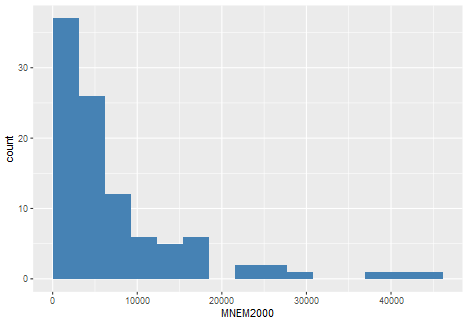
\includegraphics{R-module-4-md_files/figure-latex/gghist-1.png}

The \texttt{nclass.FD} function calculates the `ideal' number of classes
based on the ``Freedman-Diaconis'' choice, based on the Inter-quartile
range. The \texttt{boundary\ =\ 0} tells the plot to align the bins to
the y-axis (0). Let's add a smoothed frequency curve to the histogram to
show density\ldots{}

\begin{Shaded}
\begin{Highlighting}[]
\NormalTok{MNEM2000\_hist }\OtherTok{\textless{}{-}}\NormalTok{ MNEM2000\_hist }\SpecialCharTok{+} 
  \FunctionTok{geom\_density}\NormalTok{(}\FunctionTok{aes}\NormalTok{(}\AttributeTok{y =}\NormalTok{ ..scaled.. }\SpecialCharTok{*} \DecValTok{10}\NormalTok{),}
               \AttributeTok{size =} \DecValTok{1}\NormalTok{)}
\CommentTok{\# The ..scaled.. represents the density curve scaled to a}
\CommentTok{\# maximum of 1. We could just use geom\_density(), but the curve}
\CommentTok{\# is much smaller and less visible}

\CommentTok{\# We also multiplied the height of the density curve by 10}
\CommentTok{\# so it\textquotesingle{}s more visible compared to our histogram!}

\NormalTok{MNEM2000\_hist}
\end{Highlighting}
\end{Shaded}

\includegraphics{R-module-4-md_files/figure-latex/ggdensity-1.png}

We should also add lines showing mean and median

\begin{Shaded}
\begin{Highlighting}[]
\NormalTok{MNEM2000\_mean }\OtherTok{\textless{}{-}} \FunctionTok{mean}\NormalTok{(NC}\SpecialCharTok{$}\NormalTok{MNEM2000)}
\NormalTok{MNEM2000\_median }\OtherTok{\textless{}{-}} \FunctionTok{median}\NormalTok{(NC}\SpecialCharTok{$}\NormalTok{MNEM2000)}

\NormalTok{MNEM2000\_hist }\OtherTok{\textless{}{-}}\NormalTok{ MNEM2000\_hist }\SpecialCharTok{+}
  \FunctionTok{geom\_vline}\NormalTok{(}
    \FunctionTok{aes}\NormalTok{(}\AttributeTok{xintercept =}\NormalTok{ MNEM2000\_mean, }\AttributeTok{color =} \StringTok{"Mean"}\NormalTok{),}
      \AttributeTok{linetype =} \StringTok{"dashed"}\NormalTok{,}
      \AttributeTok{size =} \DecValTok{1}\NormalTok{) }\SpecialCharTok{+}
  \FunctionTok{geom\_vline}\NormalTok{(}
    \FunctionTok{aes}\NormalTok{(}\AttributeTok{xintercept =}\NormalTok{ MNEM2000\_median, }\AttributeTok{color =} \StringTok{"Median"}\NormalTok{),}
      \AttributeTok{linetype =} \StringTok{"dashed"}\NormalTok{,}
      \AttributeTok{size =} \DecValTok{1}
\NormalTok{  ) }\SpecialCharTok{+}
  \FunctionTok{scale\_color\_manual}\NormalTok{(}\AttributeTok{name =} \StringTok{"Statistics"}\NormalTok{,}
                     \AttributeTok{values =} \FunctionTok{c}\NormalTok{(}\AttributeTok{Mean =} \StringTok{"salmon"}\NormalTok{,}
                                \AttributeTok{Median =} \StringTok{"turquoise"}\NormalTok{))}

\NormalTok{MNEM2000\_hist}
\end{Highlighting}
\end{Shaded}

\includegraphics{R-module-4-md_files/figure-latex/gglabels-1.png}

Let's break down what we just did\ldots{}

First, we assigned mean and median values of \texttt{MNEM2000}~to their
respective variables. Technically, we could do this all within the
\texttt{geom\_vline()} function
(e.g.~\texttt{aes(xintercept\ =\ mean(NC\$MNEM2000)}), but this way will
make it more organized when you create plots of different variables.

The \texttt{geom\_vline()} function plots a \textbf{v}ertical
\textbf{line}, and it's possible to assign an
\texttt{xintercept}~aesthetic mapping. ``Median'' and ``Mean'' obviously
aren't colors, but we're telling our plot to use those as
``placeholder'' values that we define later, using
\texttt{scale\_color\_manual()}. Additionally, we can set the size and
linetype arguments. Normally, you can just define the color of a
\texttt{geom\_vline()} by saying something like
\texttt{color\ =\ "blue"}, but this is how to do it if you want to have
a legend describing each object.

Finally, we should add some labels and a title. Note that we could have
used all of these ggplot functions in one `section'; an example of this
will show up in the last section of this R Module.

\begin{Shaded}
\begin{Highlighting}[]
\NormalTok{MNEM2000\_hist }\OtherTok{\textless{}{-}}\NormalTok{ MNEM2000\_hist }\SpecialCharTok{+} 
  \FunctionTok{labs}\NormalTok{(}\AttributeTok{title =} \StringTok{"Descriptive Statistics of Manufacturing (2000)"}\NormalTok{,}
       \AttributeTok{x =} \StringTok{"Manufacturing Jobs"}\NormalTok{,}
       \AttributeTok{y =} \StringTok{"Count"}\NormalTok{)}

\NormalTok{MNEM2000\_hist}
\end{Highlighting}
\end{Shaded}

\includegraphics{R-module-4-md_files/figure-latex/gglabels2-1.png}

Not bad! A few things could use some work; we could change some colors,
of course, but this'll do for the time being!

\begin{enumerate}
\def\labelenumi{\arabic{enumi}.}
\tightlist
\item
  \textbf{Create a histogram (using the \texttt{nclass.FD()} function)
  with frequency (\texttt{geom\_density()}) curves, mean and median
  lines (\texttt{geom\_vline()}), appropriate axis labels, and titles
  (\texttt{labs()}) for all four employment variables. Choose your own
  colors, font, etc.!}
\end{enumerate}

If you want to arrange your four plots into a grid, refer to the
\textbf{tips and tricks} section to see how to combine plots easily in
ggplot.

\begin{center}\rule{0.5\linewidth}{0.5pt}\end{center}

\pagebreak

\hypertarget{visualizing-spatial-data-with-sf}{%
\subsection{\texorpdfstring{Visualizing spatial data with
\texttt{sf}}{Visualizing spatial data with sf}}\label{visualizing-spatial-data-with-sf}}

We already know some important things about employment variables from
reviewing visual and descriptive measures. For instance, we know that
the data to the right of the mean have a lot of observations (a high
value) for manufacturing in 2000. Since we know that this data is
aggregated at the county level (the scale of our shapefile), this means
the majority of North Carolina's 100 counties have far fewer
manufacturing jobs than the mean for the state. In other words, we have
an initial clue that jobs are distributed unevenly across the 100
counties.

This is a perfect test case for one of the descriptive spatial measures
that you were introduced to -- the \textbf{Location Quotient}~(LQ).
Let's explore how evenly (or unevenly) jobs are distributed across the
state's 100 counties. To do this, we'll use our shapefile and introduce
a new technique in R by creating a custom function to calculate the LQ
for each county in 2000.

Recall from our discussion that the LQ is a ratio of the frequency of
something within a particular area to the total frequency across a
larger set of such area. Applying this to our observations of
manufacturing jobs in NC would result in a formula like this for each
county:

\(\frac{\text{(manufacturing jobs in county)/(total jobs in county)}}{\text{(manufacturing jobs in state)/(total jobs in state)}}\)

The information that we need for the numerator of the LQ calculation is
already in our shapefile (\texttt{MNEM2000} and \texttt{TOTJOB2000}). We
need to do some preparation first to calculate the denominator.

We can do this in R by first calculating the statewide ratio of
manufacturing jobs to total job, which can be done by taking the sum of
the county-level values:

\begin{Shaded}
\begin{Highlighting}[]
\NormalTok{JOBRATE}\FloatTok{.2000} \OtherTok{\textless{}{-}} 
  \FunctionTok{sum}\NormalTok{(NC}\SpecialCharTok{$}\NormalTok{MNEM2000)}\SpecialCharTok{/}\FunctionTok{sum}\NormalTok{(NC}\SpecialCharTok{$}\NormalTok{TOTJOB2000)}

\NormalTok{JOBRATE}\FloatTok{.2000}
\end{Highlighting}
\end{Shaded}

\begin{verbatim}
## [1] 0.1144246
\end{verbatim}

Returning this new variable gives us an expected outcome of
\texttt{0.1144246} -- that is, if manufacturing jobs were evenly
distributed across North Carolina, then we'd expect manufacturing jobs
to comprise roughly 11.4\% of all jobs in a given county.

Now, we can calculate our LQ for each county by comparing it to
\texttt{JOBRATE.2000}, but we need to add a new field to our shapefile's
attribute table to hold the results. We'll create the field and populate
it with the calculated LQ values.

In base R, this can be done with:

\begin{Shaded}
\begin{Highlighting}[]
\NormalTok{NC}\SpecialCharTok{$}\NormalTok{LQ2000 }\OtherTok{\textless{}{-}}  
\NormalTok{  (NC}\SpecialCharTok{$}\NormalTok{MNEM2000}\SpecialCharTok{/}\NormalTok{NC}\SpecialCharTok{$}\NormalTok{TOTJOB2000) }\SpecialCharTok{/}\NormalTok{ JOBRATE}\FloatTok{.2000}
\end{Highlighting}
\end{Shaded}

\ldots or equally using the package \texttt{dplyr}'s \texttt{mutate()}
function and pipe operator (\texttt{\%\textgreater{}\%}) to be more
advanced!

\begin{Shaded}
\begin{Highlighting}[]
\FunctionTok{library}\NormalTok{(dplyr)}
\NormalTok{NC }\OtherTok{\textless{}{-}}\NormalTok{ NC }\SpecialCharTok{\%\textgreater{}\%}
  \FunctionTok{mutate}\NormalTok{(}\AttributeTok{LQ2000 =}\NormalTok{ (MNEM2000 }\SpecialCharTok{/}\NormalTok{ TOTJOB2000) }\SpecialCharTok{/}\NormalTok{ JOBRATE}\FloatTok{.2000}\NormalTok{)}
\end{Highlighting}
\end{Shaded}

Let's look at the results:

\begin{Shaded}
\begin{Highlighting}[]
\FunctionTok{summary}\NormalTok{(NC}\SpecialCharTok{$}\NormalTok{LQ2000)}
\end{Highlighting}
\end{Shaded}

\begin{verbatim}
##    Min. 1st Qu.  Median    Mean 3rd Qu.    Max. 
##  0.1901  0.6925  1.0055  1.0432  1.4232  2.4606
\end{verbatim}

We can actually use \texttt{sf} to write our results to a shapefile, or
even a .csv for use in Excel! Let's try it, so we can email our
shapefile to all our friends. Remember when we set our working directory
with \texttt{setwd()}? Because we did that step, we don't have to
include the entire file path now!

\begin{Shaded}
\begin{Highlighting}[]
\FunctionTok{st\_write}\NormalTok{(NC, }\StringTok{"example.shp"}\NormalTok{)}
\end{Highlighting}
\end{Shaded}

\begin{center}\rule{0.5\linewidth}{0.5pt}\end{center}

\hypertarget{choropleth-mapping-with-ggplot2}{%
\paragraph{\texorpdfstring{Choropleth mapping with
\texttt{ggplot2}}{Choropleth mapping with ggplot2}}\label{choropleth-mapping-with-ggplot2}}

Let's take the results of our analysis and generate a choropleth map. If
you want some color inspiration, try calling the \texttt{colors()}
function, which prints a list of all the colors in base R. Anyways, the
\texttt{scale\_color\_steps} and \texttt{scale\_fill\_steps} are useful
for graduated (choropleth) mapping. Remember, in ggplot, \emph{color}
represents the line color, and \emph{fill} defines the fill color. Let's
get started! Rather than do everything in multiple steps, let's call our
ggplot all in one function.

\begin{Shaded}
\begin{Highlighting}[]
\NormalTok{LQ\_2000\_gg }\OtherTok{\textless{}{-}} \FunctionTok{ggplot}\NormalTok{(}\AttributeTok{data =}\NormalTok{ NC, }\AttributeTok{mapping =} \FunctionTok{aes}\NormalTok{(}\AttributeTok{fill =}\NormalTok{ LQ2000)) }\SpecialCharTok{+}
  \FunctionTok{geom\_sf}\NormalTok{() }\SpecialCharTok{+}
  \FunctionTok{scale\_fill\_steps}\NormalTok{(}\AttributeTok{low =} \StringTok{"snow"}\NormalTok{,}
                   \AttributeTok{high =} \StringTok{"springgreen4"}\NormalTok{,}
                   \AttributeTok{n.breaks =} \DecValTok{6}\NormalTok{) }\SpecialCharTok{+}
  \FunctionTok{labs}\NormalTok{(}\AttributeTok{title =} \StringTok{"Location Quotient for Manufacturing Jobs (2000)"}\NormalTok{,}
       \AttributeTok{fill =} \StringTok{"LQ (2000)"}\NormalTok{,}
       \AttributeTok{caption =} \StringTok{"(your name here)"}\NormalTok{)}

\NormalTok{LQ\_2000\_gg}
\end{Highlighting}
\end{Shaded}

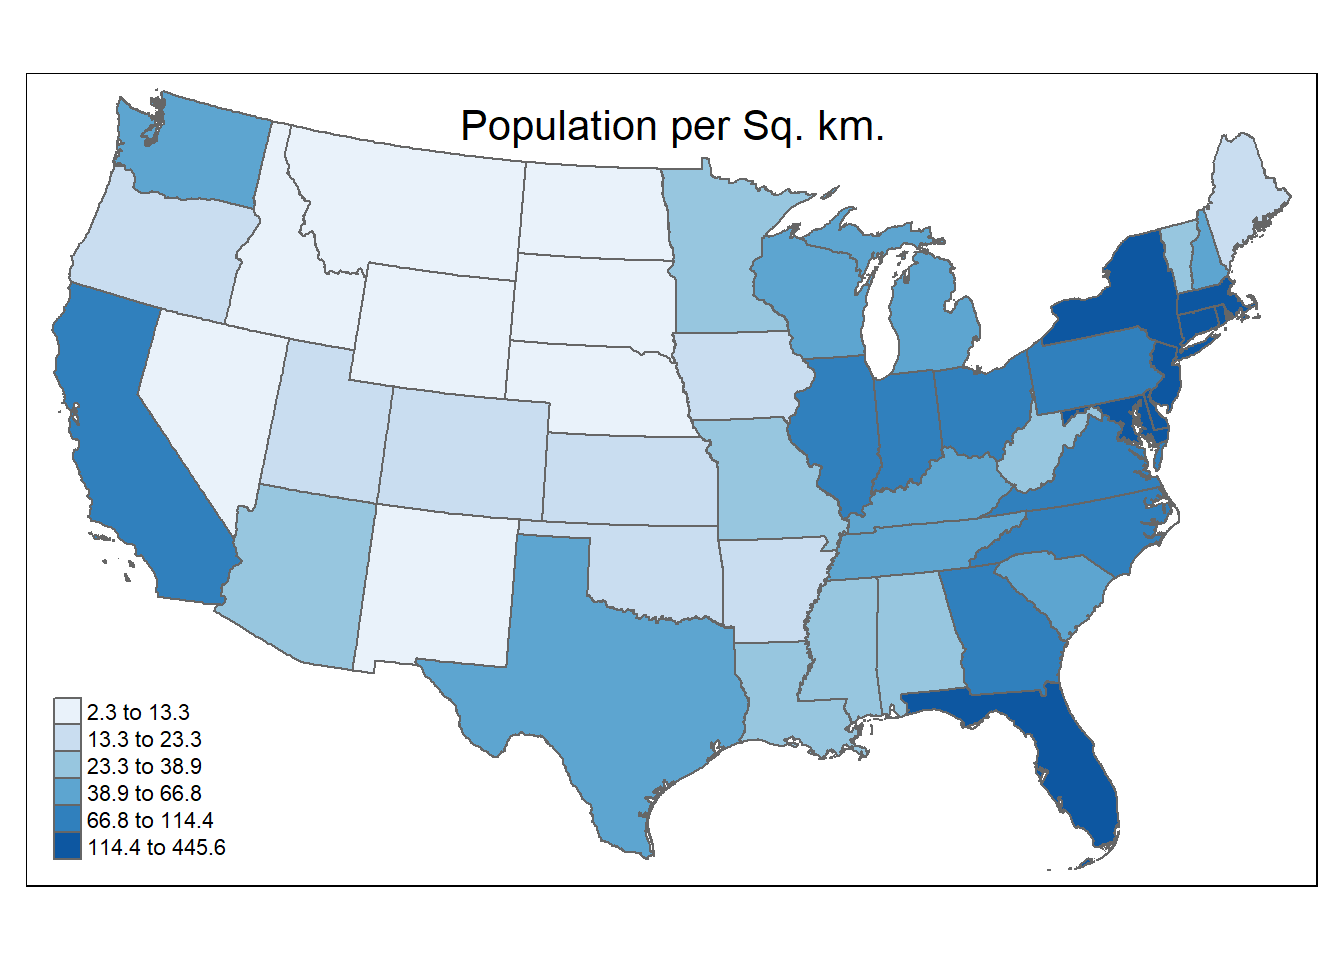
\includegraphics{R-module-4-md_files/figure-latex/choropleth-1.png}

Awesome! Now you're ready to generate your own choropleth maps in R!

\begin{enumerate}
\def\labelenumi{\arabic{enumi}.}
\setcounter{enumi}{1}
\item
  \textbf{Create and provide a map of the Location Quotient of
  manufacturing jobs in both 1990 and 2000. Provide your R code for the
  1990 map; showing how you calculated the LQ and created the map.}
\item
  \textbf{Use the \texttt{st\_write()} function to save NC to a
  shapefile where you can use it again later.}
\item
  \textbf{Using your two LQ maps, provide a short description of how
  jobs are distributed across North Carolina's counties, and how this
  changed (if at all) from 1990 to 2000.}
\end{enumerate}

Submit everything to Google Classroom!

\begin{center}\rule{0.5\linewidth}{0.5pt}\end{center}

\pagebreak

\hypertarget{tips-and-tricks}{%
\subsubsection{Tips and Tricks}\label{tips-and-tricks}}

Combining multiple plots in base R is a little tedious; you have to set
parameters for how many rows and columns of plots you want, which can be
tiresome when you're generating a lot of different plots. Fortunately,
this becomes much easier when using ggplots, thanks to the
\texttt{plot\_grid()} function in the \texttt{cowplot}~package. Assign
your ggplot to a variable (\texttt{\textless{}-}) to keep things tidy!
The \texttt{nrow}~and \texttt{ncol} arguments are optional, and
\texttt{plot\_grid} can arrange plots automatically if needed.

\begin{Shaded}
\begin{Highlighting}[]
\NormalTok{cowplot}\SpecialCharTok{::}\FunctionTok{plot\_grid}\NormalTok{(}
  \AttributeTok{plotlist =} \FunctionTok{list}\NormalTok{(example}\FloatTok{.1}\NormalTok{, example}\FloatTok{.2}\NormalTok{, example}\FloatTok{.3}\NormalTok{, example}\FloatTok{.4}\NormalTok{)}
\NormalTok{  )}
\end{Highlighting}
\end{Shaded}

\includegraphics{R-module-4-md_files/figure-latex/cowplot2-1.png}

\end{document}
